\begin{theo}[Convexity for $C^1$ functions]{ConvexityC1}
    \begin{minipage}{0.60\textwidth}
        Assume that $f: \ \Omega \rightarrow \R$ is continuously differentiable and $\Omega$ is convex. Then holds that $f$ is convex if and only if 
        \begin{equation*}
            \forall x,y \in \Omega: \ f(y) \geq f(x) + \nabla f(x)^T(y-x)
        \end{equation*}
        i\@.e\@. tangents lie below the graph.
    \end{minipage}
    \begin{minipage}{0.3\textwidth}
        \begin{center}
            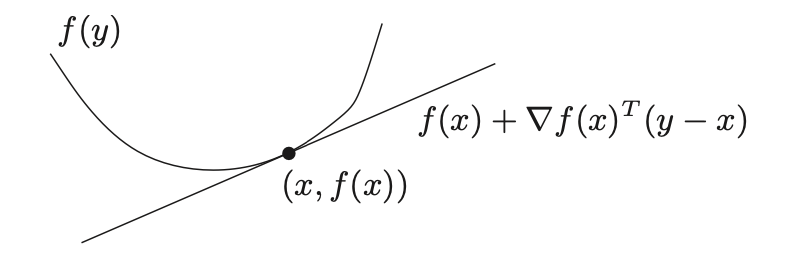
\includegraphics[scale = 0.45]{Images/Fundamental/C1Convexity.png}
        \end{center}
    \end{minipage}
\end{theo}

\begin{prf}[Convexity for $C^1$ functions]{prfConvexityC1}
    ``$\Rightarrow$'': Due to convexity of $f$ holds for given $x,y \in \Omega$  and for any $\lambda \in [0,1]$ that
    \begin{equation*}
        f(x + \lambda(y-x)) - f(x) \leq \lambda(f(y) - f(x)).
    \end{equation*}
    and therefore that 
    \begin{equation*}
        \nabla f(x)^T(y-x) 
            = \lim_{\lambda \rightarrow 0}  \frac{f(x + \lambda(y-x)) - f(x)}{\lambda}
            \leq f(y) - f(x).
    \end{equation*}

    ``$\Leftarrow$'': To prove that $z = x + \lambda(y-x) = (1-\lambda)x + \lambda y$ holds that $f(z) \leq (1-\lambda)f(x) + \lambda f(y)$, we can use the equation from Theorem~\ref{ConvexityC1} twice to get
    \begin{equation*}
        f(x) \geq f(z) + \nabla f(z)^T(x-z) \ \ \text{and} \ \ f(y) \geq f(z) + \nabla f(z)^T(y-z),
    \end{equation*}
    which yield, when weighted with $(1-\lambda)$ and $\lambda$ respectively, that
    \begin{equation*}
        (1-\lambda)f(x) + \lambda f(y) \geq f(z) + \nabla f(z)^T \underset{= 0}{\underbrace{\left[(1-\lambda)(x-z) + \lambda(y-z)\right]}}
    \end{equation*}
    \vspace{-0.75cm}
\end{prf}

\begin{theo}[Convexity for $C^2$ functions]{ConvexityC2}
    Assume that $f: \ \Omega \rightarrow \R$ is twice continuously differentiable and $\Omega$ is convex and open. Then holds that $f$ is convex if and only if
    \begin{equation*}
        \forall x \in \Omega: \ \nabla^2 f(x) \succeq 0,
    \end{equation*}
    i\@.e\@. the Hessian of $f$ is positive semi-definite.
\end{theo}

\begin{prf}[Convexity for $C^2$ functions]{prfConvexityC2}
    ``$\Rightarrow$'': Recall that a second order Taylor expansion of $y$ at $x$ in an arbitrary direction $p$ is given by the following:
    \begin{equation*}
        f(x + tp) = f(x) + t \nabla {f(x)}^T p + \frac{t^2}{2} p^T \nabla^2 f(x) p + o(t^2\|p\|).
    \end{equation*}
    From this we obtain that
    \begin{equation*}
        p^T \nabla^2 f(x) p = \lim_{t \rightarrow 0} \frac{2}{t^2} \left(\underset{(\ref*{ConvexityC1}): \ \geq 0}{\underbrace{f(x + tp) - f(x) - t \nabla {f(x)}^T p}}\right) \geq 0.
    \end{equation*}

    ``$\Leftarrow$'': Conversely, to prove the other direction, we use Theorem~\ref{TaylorRest} with some arbitrary $\theta \in [0,1]$:
    \begin{equation*}
        f(y) = f(x) + \nabla {f(x)}^T(y-x) + \underset{(\ref*{ConvexityC2}): \ \geq 0}{\underbrace{\frac{t^2}{2} {(y-x)}^T \nabla^2 f(x + \theta(y-x)) (y-x)}},
    \end{equation*}
    and thus $f$ is convex, since Theorem~\ref{ConvexityC1} trivially holds.
\end{prf}

\begin{pro}[Convexity perserving operations on convex functions]{ConvexPerservingOptsConvexFunctions}
    The following operations preserve the convexity of a function:
    \begin{enumerate}
        \item 
            Non-negative weighted sum: Suppose that $\forall i \in [i,m]: \ f_i: \R^n \rightarrow \R$ are convex functions and $\forall i \in [1,m]: \ \lambda_i \geq 0$. Then the function
                \begin{equation*}
                    f(x) = \sum_{i=1}^m \lambda_i f_i(x)
                \end{equation*}
            is convex. 
        \item 
            Affine input transformation: If $f: \ \Omega \rightarrow \R$ is convex, then also
            \begin{equation*}
                A \in \R^{n \times m}: \ \tilde{f}(x) = f(Ax + b)
            \end{equation*}
            is convex on the domain $\tilde{\Omega} = \{x \ | \ Ax + b \in \Omega\}$.
        \item 
            Concatenation with monotone convex function: If $f: \ \Omega \rightarrow \R$ is convex and $g: \ \R \rightarrow \R$ is convex and monotonely increasing, then the composition $g \circ f$ is convex.
        \item 
            Pointwise supremum: The supremum over a set of convex functions $f_i(x)$, $i \in I$, where $I$ can be an infinite set, i\@.e\@.,
            \begin{equation*}
                f(x) = \sup_{i \in I} f_i(x)
            \end{equation*}
            is convex.
        \item 
            Composition: Let $h: \R^m \rightarrow \R$ and $g: \R^n \rightarrow \R^m$ with $g = (g_1, \ldots, g_m)$. Then $f(x) = (h \circ g)(x) = h(g(x))$ is convex if any of the followings holds: 
            \begin{enumerate}
                \item 
                    $h$ is convex and non-decreasing in each argument and $\forall i \in [1,m]: \ g_i$ is convex.
                \item 
                    $h$ is convex and non-decreasing in each argument and $\forall i \in [1,m]: \ g_i$ is concave, i\@.e\@. $-g_i$ is convex.
            \end{enumerate}
    \end{enumerate}
    \vspace*{-0.2cm}
\end{pro}

\begin{prf}[Convexity perserving operations on convex functions]{prfConvexPerservingOptsConvexFunctions}
    \begin{enumerate}
        \item 
            TODO (use the definition of convexity).
        \item 
            TODO (use the definition of convexity).
        \item 
            Recall that $g$ is a convex and monotonely increasing function, then: 
            \begin{equation*}
                \nabla^2 (g \circ f) = \underbrace{g''(f(x))}_{\geq 0} \underbrace{\nabla f(x) \nabla {f(x)}^T }_{\succeq 0} + \underbrace{g'(f(x))}_{\geq 0} \underbrace{\nabla^2 f(x)}_{\succeq 0} \succeq 0,
            \end{equation*}
            i\@.e\@. $g \circ f$ is convex, since the Hessian is positive semi-definite.
        \item 
            Epigraph of $f$ is the intersection of the epigraphs of $f_i$, which are convex.
        \item
            Recall that $g_i$ is convex and that $h$ is convex and non-decreasing in each argument. Then:
            \begin{align}
                f(\lambda x + (1 - \lambda)y) 
                    &= h(g(\lambda x + (1 - \lambda)y)) \notag \\
                    &\leq h(\lambda g(x) + (1 - \lambda)g(y)) \\
                    &\leq \lambda h(g(x)) + (1 - \lambda)h(g(y)) \\
                    &= \lambda f(x) + (1 - \lambda)f(y), \notag
            \end{align}
            where we used the convexity of $g_i$ and the fact that $h$ is non-decreasing to obtain inequality (1), and the convexity of $h$ to obtain inequality (2). 
    \end{enumerate}
    \vspace*{-0.2cm}
\end{prf}

% \begin{theo}[Concave function]{Concave}
%     A function $f: \ \Omega \rightarrow \R$ is concave if and only if $-f$ is convex.
% \end{theo}

% \begin{theo}[Convex Maximization Problem]{ConvexMaximizationProblem}
%     A maximization problem
%     \begin{maxi*}|l|
%         {x \in \mathbb{R}^n}{f(x)}
%         {}{}
%         \addConstraint{x \in \Omega}.
%     \end{maxi*}
%     is called a convex maximization problem if $f$ is concave and $\Omega$ is convex. Naturally, the dual problem is then a convex minimization problem of the form 
%     \begin{mini*}|l|
%         {x \in \mathbb{R}^n}{-f(x)}
%         {}{}
%         \addConstraint{x \in \Omega}.
%     \end{mini*}
%     \vspace*{-0.5cm}
% \end{theo}

% \newpage

\begin{theo}[Convexity of Sublevel subsets]{ConvexitySublevelSubset}
    \vspace*{-0.7cm}
    \begin{minipage}{0.56\textwidth}
        If $f: \ \Omega \rightarrow \R$ is a convex function, then all its level sets 
        \begin{equation*}
            \text{lev}_{\leq \gamma}f = \{x \in \Omega \ | \ f(x) \leq \gamma\}
        \end{equation*}
        are convex.
    \end{minipage}
    \begin{minipage}{0.42\textwidth}
        \begin{center}
            \vspace*{0.2cm}
            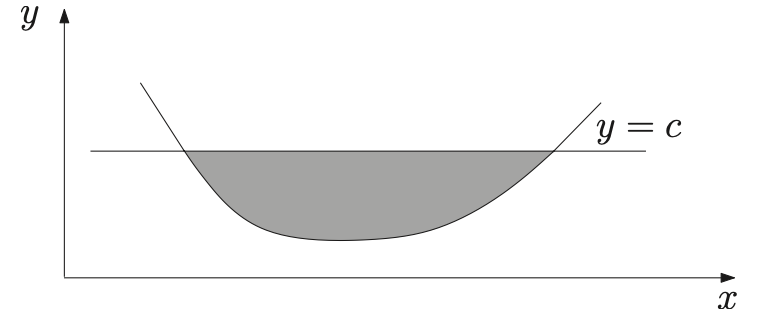
\includegraphics[scale = 0.495]{Images/Fundamental/ConvexSubset.png}
        \end{center}
    \end{minipage}
    \vspace{-0.3cm}
\end{theo}

\begin{prf}[Convexity of Sublevel subsets]{prfConvexitySublevelSubset}
    If $f(x) \leq c$ and $f(y) \leq c$, then for any $\lambda \in [0,1]$ holds also 
    \begin{equation*}
        f((1-\lambda)x + \lambda y) \leq (1-\lambda)f(x) + \lambda f(y) \leq \underset{= c}{\underbrace{(1-\lambda)c + \lambda c}}.
    \end{equation*}
    \vspace*{-0.7cm}
\end{prf}

\begin{pro}[Convexity perserving operations on convex sets]{ConvexityPreservingOperations}
    The following operations preserve the convexity of a set:
    \begin{enumerate}
        \item The intersection of finitely or infinitely many convex sets is convex.
        \item Affine image: if $\Omega$ is convex, then for $A \in \R^{m \times n}$, $b \in \R^m$ also the set $A\Omega + b = \{ y \in \R^m \ | \ \exists x \in \Omega : y = Ax + b \}$ is convex.
        \item Affine pre-image: if $\Omega$ is convex, then for $A \in \R^{n \times m}$, $b \in \R^n$ also the set $\{ z \in \R^m \ | \ Az + b \in \Omega \}$ is convex.
    \end{enumerate}
\end{pro}

\begin{ex}[Convex Feasible set]{ConvexFeasibleSet}
    If $\forall i \in [1,m]: f_i : \ \R^n \rightarrow \R$ are convex functions, then the set 
    \begin{equation*}
        \Omega = \{x \in \R^n \ | \ f_i(x) \leq 0, \ i \in [1,m]\}
    \end{equation*}
    is a convex set, because it is the intersection of sublevel sets $\Omega_i$ of convex functions $f_i$, i\@.e\@.
    \begin{align*}
        \Omega 
            &= \bigcap_{i=1}^m \Omega_i \\
            &= \bigcap_{i=1}^m \ \{x \in \R^n \ | \ f_i(x) \leq 0 \}.
    \end{align*}
    \vspace{-0.5cm}
\end{ex}


\begin{theo}[Optimality condition for convex problems]{OptimalityConditionConvexProblems}
    Regard a convex optimization problem with continuously differentiable objective function $f$. A point $x^* \in \Omega$ is a global optimizer if and only if 
    \begin{equation*}
        \forall y \in \Omega: \ \nabla {f(x^*)}^T(y - x^*) \geq 0.
    \end{equation*} 
    \vspace*{-0.5cm}
\end{theo}

\newpage

\begin{prf}[Optimality condition for convex problems]{prfOptimalityConditionConvexProblems}
    ``$\Rightarrow$'': Assume for the sake of contradiction that $\exists y \in \Omega: \ \nabla {f(x^*)}^T(y - x^*) < 0$, then we could regard a Taylor expansion
    \begin{equation*}
        f(x^* + \lambda(y - x^*)) = f(x^*) + \lambda \underbrace{\nabla {f(x^*)}^T(y - x^*)}_{<0} + \underbrace{o(\lambda)}_{\rightarrow 0}.
    \end{equation*}
   This implies that for sufficiently small positive $\lambda$, we have 
   \begin{equation*}
        f(x^* + \lambda(x - x^*)) < f(x^*),
   \end{equation*}
   which contradicts the optimality of $x^*$. \\

    ``$\Leftarrow$'': 
   Due to the $C^1$ characterization of convexity of $f$ in Theorem~\ref{ConvexityC1}, we have for any feasible $y \in \Omega$: 
   \begin{equation*}
       f(y) \geq f(x^*) + \underbrace{\nabla {f(x^*)}^T(y - x^*)}_{\geq 0} \geq f(x^*),
   \end{equation*}
   which implies that $x^*$ is a global optimizer.
\end{prf}  

\begin{theo}[Sufficient Condition for Convex NLP]{SufficientConditionConvexNLP}
    For a nonlinear optimization problem (NLP) in standard form
    \begin{mini*}|l|
        {x \in \R^n}{f(x)}
        {}{}
        \addConstraint{g_i(x) = 0, \ }{i \in [1,m]}
        \addConstraint{h_i(x) \geq 0, \ }{j \in [1,p]},
    \end{mini*}
    the following conditions are necessary for convexity:
    \begin{itemize}
        \item 
            the objective function $f: \R^n \rightarrow \R$ must be convex,
        \item 
            the constraint set 
            \begin{equation*}
                X = \{ x \in \R^n \ | \ g(x) = 0,\ h(x) \geq 0 \}
            \end{equation*}
            must be convex. Since we know that the intersection of convex sets is convex, we can write $X$ as the intersection of the sets $G$ and $H$:
            \begin{align*}
                X 
                    &= \{ x \in \R^n \ | \ g(x) = 0,\ h(x) \geq 0 \} \\ 
                    &= \{x \in \R^n \ | \ g(x) = 0\} \cap \{x \in \R^n \ | \ h(x) \geq 0\} \\ 
                    &= \left( \bigcap_{i=1}^m \{x \in \R^n \ | \ g_i(x) = 0\} \right) 
                    \ \cap \
                    \left( \bigcap_{i=1}^m \{x \in \R^n \ | \ h_i(x) \geq 0\} \right) \\ 
                    &= G \cap H
            \end{align*}
            Now we must consider the requirements for the sets $G$ and $H$ to be convex:
            \begin{itemize}
                \item 
                    Suppose $-H_i = \{x \in \mathbb{R}^n \mid h_i(x) \leq 0\}$, the zero sublevel set of the function $h_i$. If $h_i$ is convex, the set $-H_i$ is convex, as seen in Theorem~\ref{ConvexitySublevelSubset}. Now, consider the case where $h_i$ is concave. Since $h_i$ being concave means that $-h_i$ is convex, the set $H_i = \{x \in \mathbb{R}^n \mid h_i(x) \geq 0\}$ is a sublevel set of the convex function $-h_i$, and is therefore convex.
                    Thus, the set $H_i$ is convex when $h_i$ is concave.
                \item            
                    On the other hand, $G$ is the level set of of $g_i$. Therefore it is certainly a convex set whenever $g_i$ is a affine function
                    \begin{equation*}
                        \forall i \in [i,m]: \ g_i(x) = a_i^T x + b_i.
                    \end{equation*} 
                \end{itemize}
        \end{itemize}
\end{theo}

\begin{ex}[Halfspace]{HalfSpace}
    A halfspace 
    \begin{equation*}
        H_{\leq} = \{ x \in \R^n \ | \ a^T x \leq b \}
    \end{equation*}
    is a convex set, as the zero sublevel set of the affine (and therefore convex) function $f(x) = a^T x - b$, cf. Theorem~\ref{ConvexitySublevelSubset}. \\

    \textbf{Note:} The opposite is not true; a function that has all its level sets convex is not necessarily convex.
\end{ex}

\begin{ex}[Polyhedral Set]{PolyhedralSet}
    A polyhedral set $C \subset \R^n$ is defined as the intersection of a finite number of halfspaces, i\@.e\@.,
    \begin{equation*}
        C = \bigcap_{i= 1, \ldots, m} \{ x \in \R^n \ | \ a_i^T x \leq b_i \}.
    \end{equation*}
    Since the intersection of convex sets is convex, $C$ is a convex set if all the halfspaces are convex. \\

    \textbf{Note:} A polyhedral set might contain equalities, i\@.e\@., 
    \begin{equation*}
        C = \{ x \in \R^n \ | \ Ax \leq b, \ Cx = d \}.
    \end{equation*}
    which can be written with just inequalities as such:
    \begin{equation*}
        C = \{ x \in \R^n \ | \ Ax \leq b, \ Cx \leq d, \ -Cx \leq -d \}.
    \end{equation*}
    \vspace*{-0.5cm}
\end{ex}

\begin{ex}[Ellipsoid]{Ellipsoid}
    If $P \in \R^{n \times n}$ is symmetric positive definite, then the ellipsoid
    \begin{equation*}
        C = \{ x \in \R^n \ | \ {(x-x_c)}^T P^{-1} (x-x_c) \leq 1 \}
    \end{equation*}
    is convex, as the $1$-sublevel set of the convex function $f(x) = {(x-x_c)}^T P^{-1} (x-x_c) - 1$, where $x_c$ is the center of the ellipsoid and $P$ is the shape matrix. The latter determines how far the ellipsoid extends in each direction from $x_c$; the lengths of the semi-axis are given by $\sqrt{\lambda_i}$, where $\lambda_i$ are the eigenvalues of $P$, while the eigenvectors of $P$ determine the orientation of the ellipsoid. When $P = r^2I$, the ellipsoid is a ball with radius $r$ around $x_c$, i\@.e\@.,
    \begin{equation*}
        C = \{ x \in \R^n \ | \ \|x - x_c\|_{2} \leq r \},
    \end{equation*}
    or, in general, the $p$-norm ball
    \begin{equation*}
        C = \{ x \in \R^n \ | \ \|x - x_c\|_{p} \leq r \}.
    \end{equation*}
    where the value of $p$ determines the shape of the ball, i\@.e\@.,
    \vspace*{0.3cm}

    \begin{itemize}
        \begin{minipage}{0.33\textwidth}
            \item 
                $p = 1$: 
                \begin{center}
                    \hspace{-1.5cm}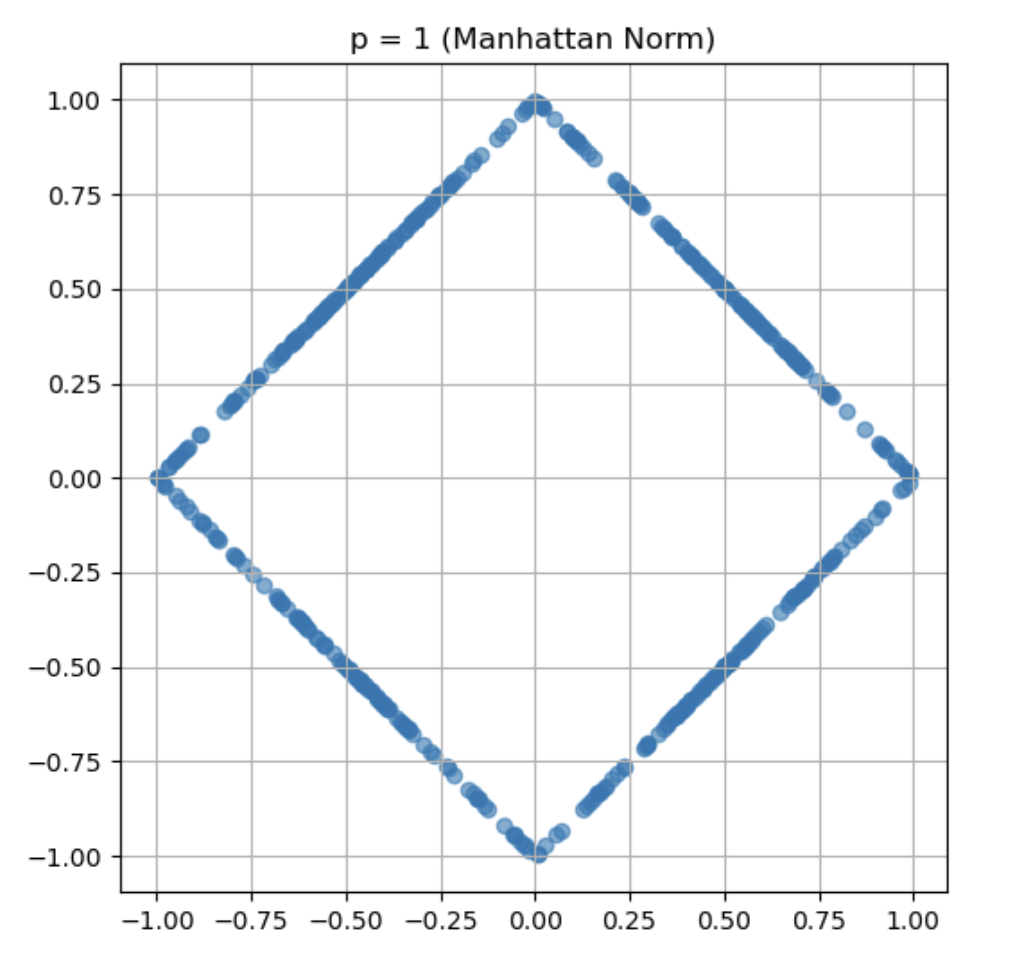
\includegraphics[scale = 0.2]{Images/Fundamental/ManhattanBall.png}
                \end{center}
        \end{minipage}
        \begin{minipage}{0.33\textwidth}
            \item 
                $p = 2$: 
                \begin{center}
                    \hspace{-1.5cm}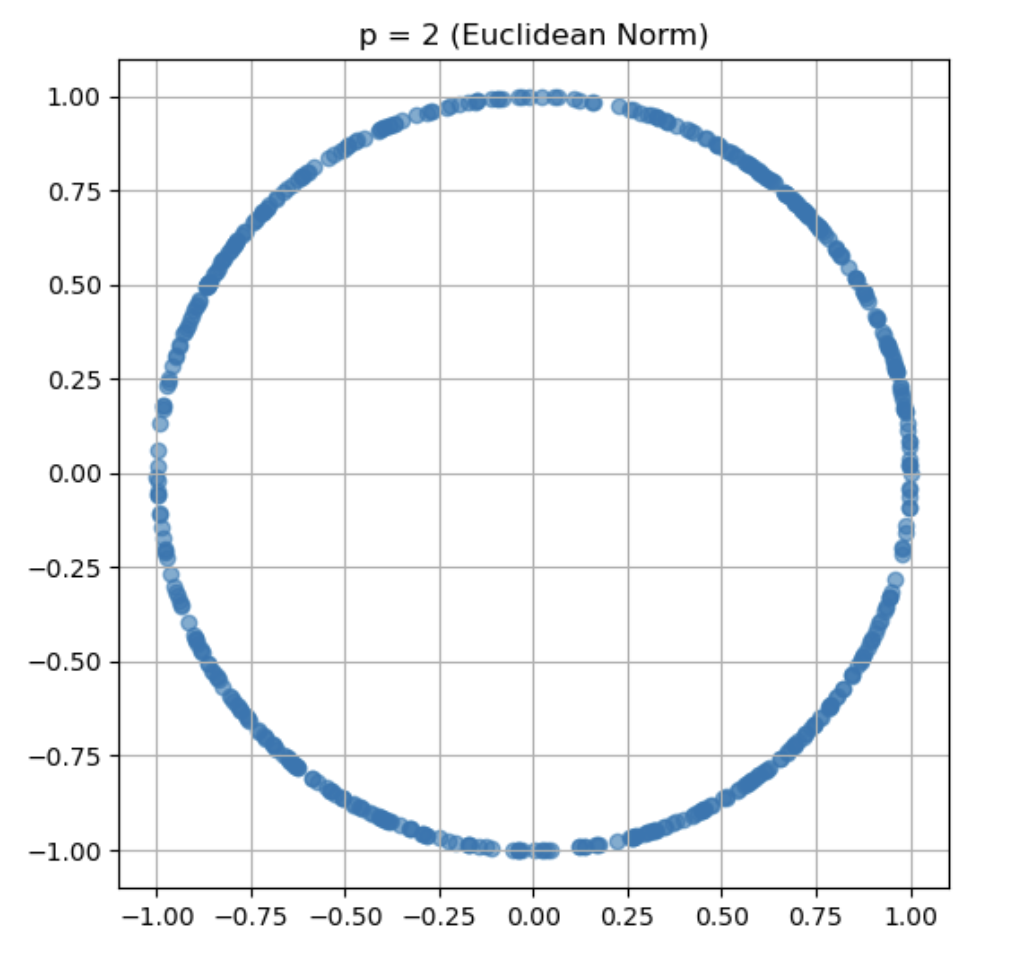
\includegraphics[scale = 0.2]{Images/Fundamental/EuclideanBall.png}
                \end{center}
        \end{minipage}
        \begin{minipage}{0.33\textwidth}
            \item 
                $p = \infty$: 
                \begin{center}
                    \hspace{-1.5cm}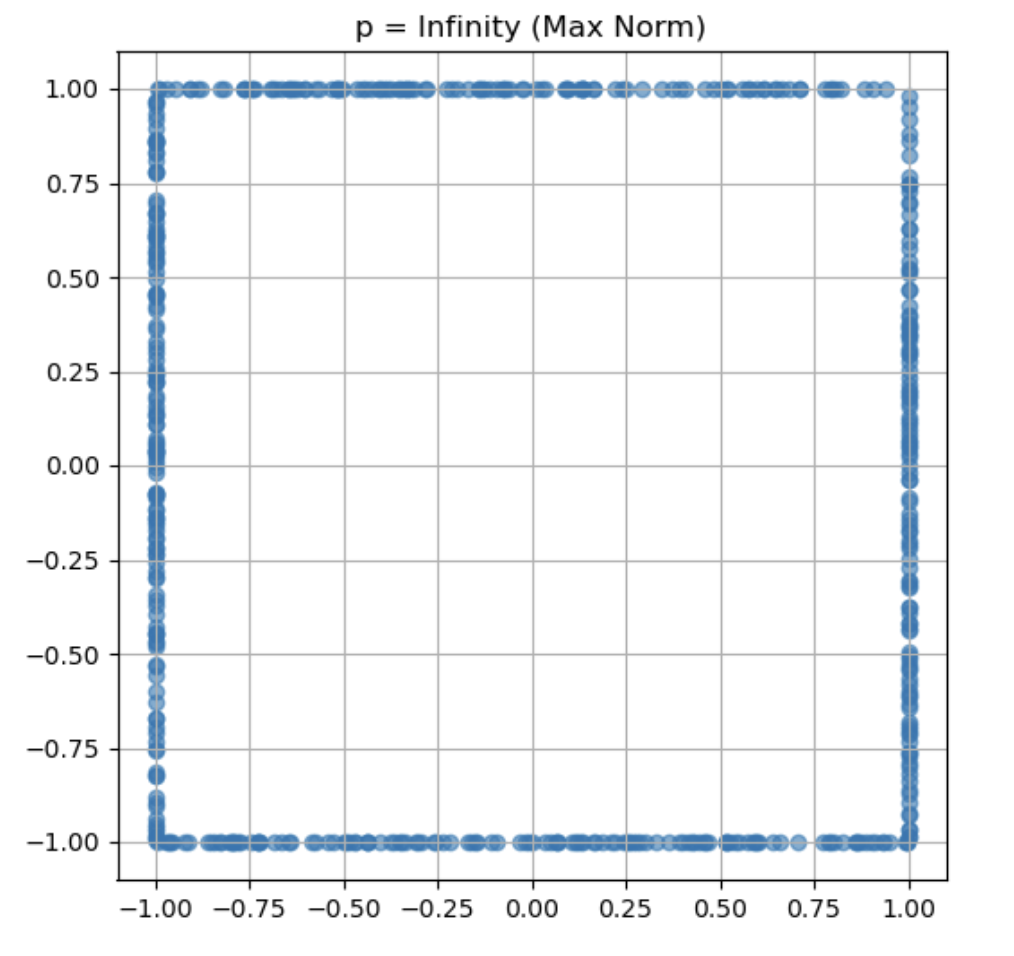
\includegraphics[scale = 0.2]{Images/Fundamental/MaxBall.png}
                \end{center}
        \end{minipage}
    \end{itemize}

    \textbf{Note:} All images above are for $r = 1$.
\end{ex}

\begin{ex}[Convex cones]{Convex cones}
    A set $C$ is said to be cone if
    \begin{equation*}
        \forall x: \ x \in C \ \Rightarrow \ \forall \lambda \geq 0: \ \lambda x \in C.
    \end{equation*}
    Moreover, $C$ is a convex cone if and only if it is closed under addition and multiplication with non-negative scalars, i\@.e\@.,
    \begin{equation*}
        \forall x,y \in C, \ \forall \lambda, \mu \geq 0: \ \lambda x + \mu y \in C.
    \end{equation*}
    \begin{minipage}{0.66\textwidth}
        The following are examples of convex cones:
        \begin{itemize}
            \item 
                Non-negative orthant: The set $C = \{ x \in \R^n \ | x \geq 0 \}$ is a convex cone. 
            \item
                Norm cones: The set $C = \{ (x,t) \in \R^n \times \R \ | \ \|x\|_p \leq t \}$ is a convex cone. For instance, the Lorenz cone or ice-cream cone, when $p = 2$, is shown on the right.
            \item Positive semi-definite cone: The set $\mathbb{S}^n_+$ is a convex cone.
        \end{itemize}
    \end{minipage}
    \begin{minipage}{0.32\textwidth}
        \vspace{0.3cm}
        \begin{center}
            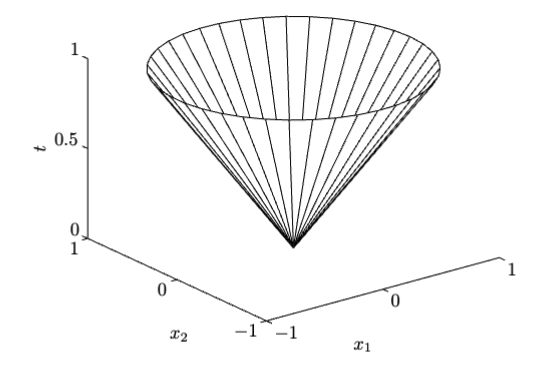
\includegraphics[scale = 0.25]{Images/Fundamental/LorenzCone.png}
        \end{center}
    \end{minipage}
\end{ex}



